\chapter{Design}\label{Design}

This chapter defines the challenges associated with the research problem and presents a refined solution. We then delve deeper into the individual components to explore the reasoning and considerations that produced this design, and outline the benefits and limitations of alternative approaches. The chapter aims to showcase this idea independent of implementation, instead using generalised concepts that may be applied by the reader within their own practice.



\section{Problem Overview}

As we saw in Chapter~\ref{Introduction}, a distributed deployment model for ECH exhibits some desirable qualities but also constitutes quite a complicated problem to solve. There are many factors at play, particularly around orchestrating TLS server co-operation, publishing ECHConfig values associated with specific servers, instructing TLS client behaviour and impeding traffic analysis attacks. Furthermore, these have to function within the confines of our imperfect world where we must accept headaches of technological inertia and legacy systems. This has only grown in prevalence on the Internet, with backbone technologies like IPv4, DNS and HTTP requiring countless workarounds or extensions to meet our modern demands without breaking backwards-compatibility.

The overall form of the solution appears somewhat similar to how conventional ECH in Split Mode operates. In Section~\ref{split-mode-deployment}, it was highlighted how Split Mode provides a means to separate ECH-service providers from private domain origin servers, but makes no attempt to remain secure when deployed across a public network nor facilitate a multi-provider setup. The approach taken here differs primarily in that the DNS resource records for a private domain can point to any IP address in the co-operative network while all co-operating TLS servers are linked together over public channels. We can see such a scenario depicted in Fig.~\ref{distributed_ech_figure}, where when examining Split Mode previously we saw three origin servers accessible through a single provider, we can now envision a client capable of querying any of the three origin servers for a private domain and having their connection transparently reach through to the correct origin server.

\begin{figure}[ht]
\centerline{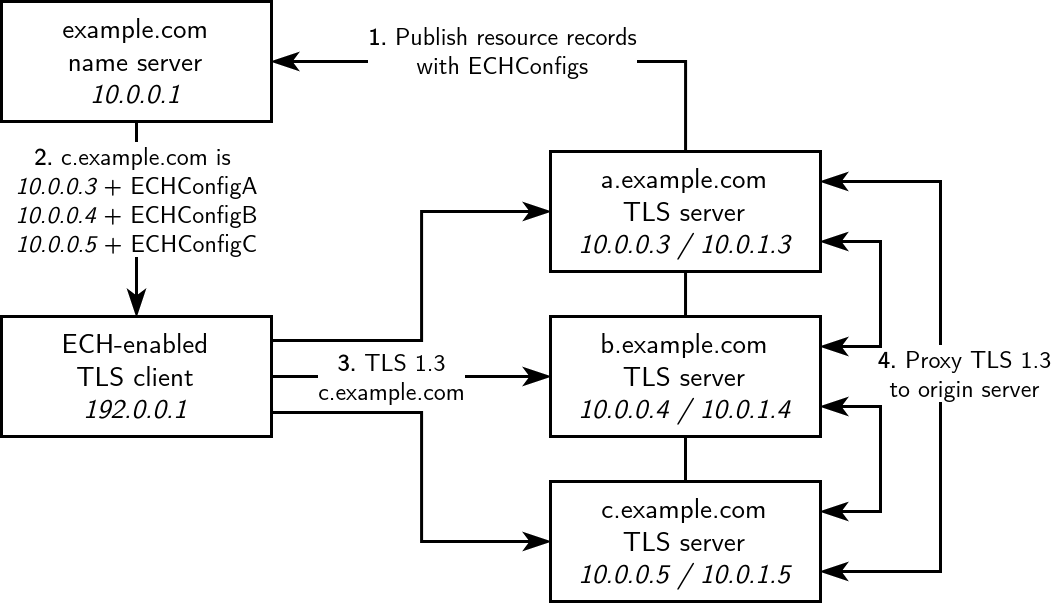
\includegraphics[width=160mm]{images/distributed-ech.png}}
\caption[Example distributed ECH deployment]{An example distributed deployment of ECH using the proposed solution. Steps 1 and 2 are completed out-of-band while steps 3 and 4 result in a TLS connection being established between the client and appropriate origin server through another TLS server.}
\label{distributed_ech_figure}
\end{figure}

This diagram hides some technical details and considerations that should be kept in mind. This loose network of TLS servers somehow need to publish DNS resource records for all private domains that can point at any one of them while referencing the corresponding ECHConfig value. Additionally, one design criteria is for load to be allocated across the network in a reasonably fair manner, so it is expected that every server is continuously operating as an ECH-service provider for other servers. As such, it is not enough to regularly cycle through sets of DNS resource records pointing towards each server one at a time but we must instead find a method to have the same DNS query uniformly spread clients amongst participating servers. This is especially hard if we want all servers to have distinct private keys and thus different ECHConfig values, as now we need to somehow associate this value with an individual server rather than with the domain name, which is a historically difficult challenge in DNS.

As both the client-server and server-server channels are over public networks, this reveals a perfect attack surface for any network observers to perform a correlation attack between server ingress and egress traffic. Even after an origin server completes the TLS handshake and establishes end-to-end encrypted communication with a client, an eavesdropper can deduce which origin server the client is interacting with by comparing ingress/egress times and packet counts.

To address these challenges, the design has been split into two topics of interest: Identifying mechanisms needed for enabling distributed deployment and disrupting correlation attacks using traffic obfuscation techniques.






\section{Distribution Mechanisms}

The previous section raised a number of criteria that must be fulfilled to allow for this distributed deployment model, which can be summarised into two points. Firstly, the solution requires a series of procedures that enables the use of DNS resource records to direct ECH-enabled clients evenly between all co-operating TLS servers with correct ECHConfig values when resolving private domain names using encrypted DNS. Then, these servers need to be able to forward client connections to each other over a public network without exposing the decrypted ClientHelloInner.

\subsection{DNS Publication Schema}

We can take advantage of the commonly seen round-robin DNS technique to share load throughout the co-operative network. Round-robin DNS works by responding to DNS queries with multiple valid IP addresses in a random order from which the client selects one. This is typically used to provide simplistic uniform load distribution without the need for dedicated load balancing software or hardware. By installing the IP addresses of all co-operating TLS servers into all private domain name DNS resource records, clients who resolve any of these domains will be directed any one of the servers. This has the additional benefit of allowing clients to immediately retry a connection with the next IP if the connection fails, although some clients might not implement this. However, a major flaw with this approach is requiring all servers to share an ECH private key because there is no way to specify which ECHConfig value should be used by the client when it selects an IP address. As such, this mechanism can only work if there is exactly one ECHConfig value to choose from.

If we are not limited to static declaration of DNS resource records, a better method can be employed here using a dynamic DNS service. We use software to regularly substitute private domain name DNS resource records such that load is fairly balanced across servers. This allows us to specify specific IP address and ECHConfig value pairs for each domain name, alleviating the need for sharing private keys. Such software can also make intelligent decisions based on real-time information such as amount of DNS queries or even reported TLS server traffic flow, which could greatly improve the fairness offered by the load balancing system in cases of heterogeneous server capabilities. Unfortunately, using dynamic DNS for load balancing is prone to sporadic inconsistency due to DNS response caching. Not only can stale cache entries send traffic to wrong locations, this can suddenly result in more traffic appearing on one IP address if a busy recursive resolver chooses to cache a response for many stub resolvers to use. Lowering the Time-To-Live (TTL) of DNS resource records may help, at the cost of more frequent polling.

It may also be worthwhile to investigate HTTPS resource records ``alternative endpoint'' functionality, which may be able to associate ECHConfig values with individual servers rather than domain names. However, this project was not able to get consistent results across different platforms with these.

\subsection{TLS Server Co-operation}

Due to servers operating as both an own origin server for their own domains and as an ECH-service provider for all other domains in the anonymity set, they need to accept both regular ClientHello messages and ClientHello messages containing the ECH extension with an encrypted ClientHelloInner. While a regular ClientHello message results in the usual TLS handshake, after decryption a ClientHelloInner can lead to either ECH in Shared Mode or Split Mode. In Shared Mode, the ClientHelloInner can now be processed as a regular ClientHello message, but Split Mode requires the server proxy the TLS connection the appropriate origin server.

When forwarding this connection to the origin server, the ClientHelloInner is now sent as a regular ClientHello without any security, entirely defeating the purpose of ECH. To solve this issue, server-server communication have some form on encryption to maintain the confidentiality of the ClientHelloInner. As widely shared secrets should be avoided and we would like this co-operation network to remain adaptable to change, a KEM and KDF backed by public key cryptography should be considered to establish ephemeral shared secrets between servers for conducting symmetric encryption.






\section{Traffic Obfuscation}

In addition to protecting the ClientHelloInner from exposure, this design also seeks to prevent revelation of which origin server a client is communicating with, as such knowledge could significantly reduce or eliminate the anonymity set cloaking the target domain name. We have already seen in Section~\ref{traffic-correlation-attacks} that ECH is susceptible to traffic correlation attacks through machine learning classifier models and that there exists many metrics useful for traffic pattern recognition. Then in the following section, it was noted that low-latency network systems are especially vulnerable to timing analysis attacks. Together, these present a difficult challenge for ensuring the security of ECH when using distributed deployment.

\begin{figure}[ht]
\centerline{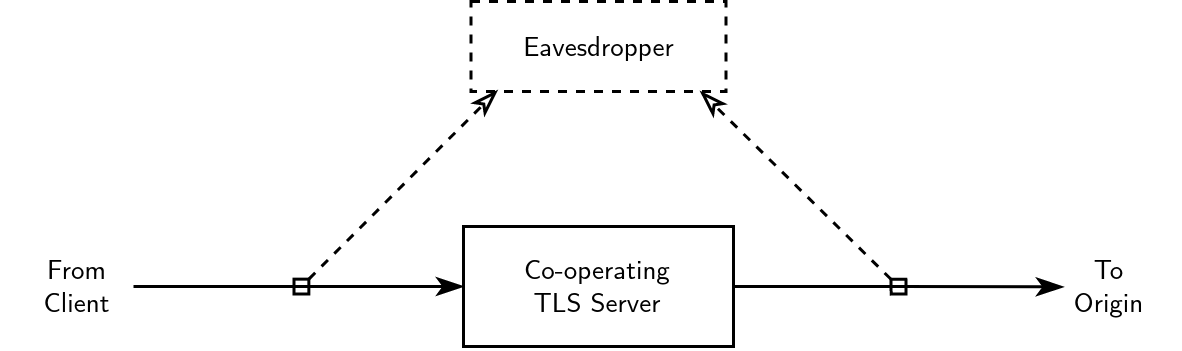
\includegraphics[width=150mm]{images/correlation-attack.png}}
\caption[Diagram of how a correlation attack can be used]{A network observer with view a of client-server and server-server channels has the opportunity to launch correlation attacks.}
\label{correlation_figure}
\end{figure}

In an attempt to mitigate these attacks, this design introduces obfuscation on top of encryption into all server-server channel traffic. These techniques are based on the goal of minimising features and interrupting patterns that occur in communication systems that can be used to find associations between channels. As seen in Fig.~\ref{correlation_figure}, if an eavesdropper can record both the ingress and egress traffic of a co-operating server, they may be able to track the movement of packets from one channel to another due to these conspicuous traits. Such a situation is not improbable, as in reality both channels are likely to pass through the same physical infrastructure or organisation at some point.

\subsection{Normalisation}

Normalisation is the process of morphing arbitrary traffic network such that a given metric remains a fixed value over time. For example, instantaneous throughput could be considered an aspect of traffic that can be correlated with another the activity in another channel. Normalisation can apply traffic shaping rules and inject noise to ensure their is a constant amount of throughout at any one time. Normalisation for masking the absence of traffic can be somewhat impractical for use in civilian-settings as bandwidth can be both limited and variable, so it might not be an economic viable approach.

\subsection{Pacing and Mixing}

While not perfect, many practical techniques exist to mask traffic with minimal impact to overall network performance. For instance, the lengths of packets may be rounded to the next multiple of 32 or such that it blends in with surrounding activity~\cite{yu2012predicted}. To disrupt timing-based correlation attacks, delays and packet slotting can be used to pace the rate of traffic. Traffic mixing, where dummy traffic is introduced into the stream, has also proven to be effective when used in conjunction with variable inter-arrival times~\cite{fu2003analytical, fu2003effectiveness}.






\section{Summary}

Every co-operating TLS server operates both as ECH-service provider for all other members and as an origin server for any domains it serves. Round-robin static DNS and dynamic DNS can be used with the HTTPS resource record to fairly distribute ECH-enabled client traffic amongst these servers, but the round-robin technique requires all servers to shared a private key. Without intervention, passive observers would be able to read ClientHelloInner values from server-server channels and undermine anonymity sets through traffic correlation. To solve this, server-server communication is encrypted and further obfuscated using traffic pacing and dummy packet mixing.
